\documentclass{article}
% translate with >> pdflatex -shell-escape <file>

% This file is used as unit test for pgfplots, copyright by Christian Feuersaenger.
% 
% See
%   http://pgfplots.sourceforge.net/pgfplots.pdf
% for pgfplots.
%
% Any required input files (for <plot table> or <plot file> or the table package) can be downloaded
% at
% http://www.ctan.org/tex-archive/graphics/pgf/contrib/pgfplots/doc/latex/
% and
% http://www.ctan.org/tex-archive/graphics/pgf/contrib/pgfplots/doc/latex/plotdata/

\usepackage{pgfplots}
\pgfplotsset{compat=newest}

\pagestyle{empty}

\begin{document}


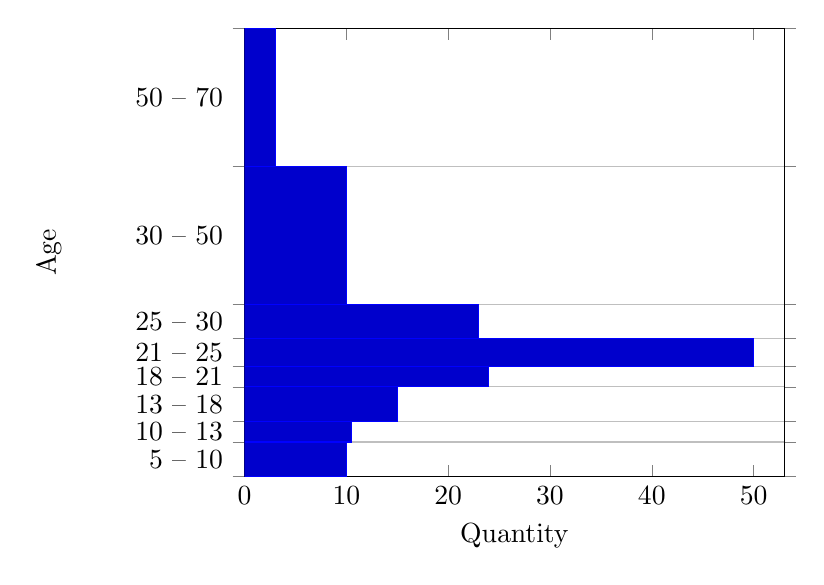
\begin{tikzpicture}
	\begin{axis}[
	xmin=0,xmax=53,
		ylabel=Age,
		xlabel=Quantity,
		y label style={yshift=0.7cm},
		enlargelimits=false,
		ytick={5,10,13,18,21,25,30,50,70},
		yticklabel={$\pgfmathprintnumber{\tick}$ -- $\pgfmathprintnumber{\nexttick}$},
		xbar interval,
	]
	\addplot[draw=blue,mark=none,fill=blue!80!black]
		plot coordinates {(10,5) (10.5,10) (15,13) (24,18) (50,21) (23,25) (10,30) (3,50) (3,70)};
	\end{axis}
\end{tikzpicture}
\end{document}
